\documentclass[letterpaper]{report}
\author{Prof. Rob Marano}
\usepackage{expl3}
\usepackage[margin=0.75in]{geometry}
\usepackage{amsfonts}
\usepackage{amsthm}
\usepackage{latexsym}
\usepackage{amsmath}
\usepackage{amssymb}
\usepackage{setspace}
\usepackage[normalem]{ulem}
\usepackage{multicol}
\usepackage{multirow}
\usepackage{bytefield}
\usepackage{color}
\usepackage{xcolor}
\usepackage{listings}
\usepackage{chronology}
\usepackage{pdfpages}
\usepackage{forloop}
\usepackage{xparse}
\usepackage{xstring}
\usepackage{listofitems}
\usepackage{courier}
\usepackage{textcomp}
\usepackage{graphicx}
\usepackage{hyperref}
\usepackage{enumerate}

\usepackage{./code/mips}
%
% mycommands.tex
%

\newcommand{\colorbitbox}[4][lrbt]{%
    \rlap{\bitbox[#1]{#3}{\color{#2}\rule{\dimexpr\width-0.4pt}{\dimexpr\height-0.4pt}}}%
    \bitbox[#1]{#3}{#4}}

\definecolor{lightgray}{gray}{0.85}

%
% \ExplSyntaxOn
% \NewDocumentCommand{\loopBin}{m}
%  {
%   % save the input in a variable
%   \tl_set:Nn \mips_getletters { #1 }
%   % replace spaces with \textvisiblespace
%   \tl_replace_all:Nnn \mips_getletters { ~ } { \textvisiblespace }
%   % map the input surrounding each item by parentheses
%   \tl_map_inline:Nn \mips_getletters { ##1 }
%  }
% \tl_new:N \mips_getletters
% \ExplSyntaxOff
%


%
% \newcommand{\binLoop}[1]
% {
%     \begin{bytefield}[boxformatting={\centering\itshape},bitwidth=1.5em,endianness=big]{32}
%     \bitheader{0-31}
%     % \StrLen{#1}
%     \foreach \x in {1,...\StrLen{#1}}
%     {
%         \bitbox{\x,#1{\x}}
%     }
    
%     \end{bytefield}
% }
%

%
 % \NewDocumentCommand{\extract}{mm}
\ExplSyntaxOn
\cs_new:Npn \extract #1 #2
 {
  \str_item:fn { #1 } { #2+1 } % since it starts counting from 1
 }
\cs_generate_variant:Nn \str_item:nn {f}
\ExplSyntaxOff

\ExplSyntaxOn
% \cs_new:Npn \makebitboxes #1 #2
 \NewDocumentCommand{\makebitboxes}{mm}
 {
    \begin{bytefield}[boxformatting={\centering\itshape},bitwidth=1.5em,endianness=big]{\numbits}
    \bitheader{0-{#1 - 1}} \\
    
    \int_step_variable:nnnNn {0}{1}{#1-1}{\tvar}
   {
        % (\tvar,\extract{#2}{\tvar})
        \int_compare:nNnTF { \int_mod:nn {\tvar} { 2 } } = { 0 }
       {% odd box
            \colorbitbox{lightgray}{1}{\extract{#2}{\tvar}}
       }
       { %even box
            \bitbox{1}{\extract{#2}{\tvar}}
       }
   }
   \end{bytefield}
  }
\ExplSyntaxOff
%

\ExplSyntaxOn
% \cs_new:Npn \makebitboxes #1 #2
 \NewDocumentCommand{\makeemptybyteboxes}{m}
 {
    \begin{bytefield}[boxformatting={\centering\itshape},bitwidth=1.5em,endianness=big]{32}
    
    \int_step_variable:nnnNn {0}{1}{#1-1}{\tvar}
   {
        % (\tvar,\extract{#2}{\tvar})
        \int_compare:nNnTF { \int_mod:nn {\tvar} { 2 } } = { 0 }
       {% odd box
            \colorbitbox{lightgray}{4}{}
       }
       { %even box
            \bitbox{4}{}
       }
   }
   \end{bytefield}
  }
\ExplSyntaxOff
%

\ExplSyntaxOn
 \NewDocumentCommand{\makeemptybitboxes}{m}
 {
    \begin{bytefield}[boxformatting={\centering\itshape},bitwidth=1.5em,endianness=big]{\numbits}
    \bitheader{0-{#1 - 1}} \\
    
    \int_step_variable:nnnNn {0}{1}{#1-1}{\tvar}
   {
        % (\tvar,\extract{#2}{\tvar})
        \int_compare:nNnTF { \int_mod:nn {\tvar} { 2 } } = { 0 }
       {% odd box
            \colorbitbox{lightgray}{1}{}
       }
       { %even box
            \bitbox{1}{}
       }
   }
   \end{bytefield}
  }
\ExplSyntaxOff
%
\input{./code/lauracode}
\input{./code/testpoints}

\hypersetup{
    colorlinks=true,
    linkcolor=blue,
    filecolor=magenta,      
    urlcolor=cyan,
    pdftitle={ECE 251 Spring 2026 Mid-Term Exam Solution Key},
    pdfpagemode=FullScreen,
}
\urlstyle{same}

\pagestyle{empty}
\begin{document}

% *** COVER *** 
\hfill {\bf Name: } {\color{red} \textbf{ANSWER KEY}}

\vspace{0.1in}

\centerline{\huge \bf Mid-Term Exam Solutions}
\vspace{0.1in}

ECE 251 \textemdash{ Computer Architecture} \hfill
12 March 2026 \hfill

Spring 2026 \hfill
Prof. Rob Marano \hfill

\vspace{0.1in}
\textsc{Read all of the following information before starting the exam:}
\begin{itemize}
	\item You have \textbf{120 minutes} for this exam, which has six (6) problems and is worth a total of \textbf{100 points}.  It is your responsibility to make sure that you answer all the problems and provide those answers in this packet. The exam is closed-book, but you have the use of the MIPS ``Green Sheet" at the end of this packet. Provide full solutions directly below the question on this handout. Keep the handout packet stapled. Loose sheets will not be accepted. Show all work, clearly and in order, if you want to get full credit.  Points will be deducted if you do not show how you arrived at your answer (even if your final answer is correct). Justify your answers with explicit assumptions whenever possible to ensure full credit. Sketch all relevant graphs and explain all relevant computations. {\bf Circle} or {\bf box} your final answer for each problem in order to {\bf indicate}, when applicable. Please keep your written answers brief, usually no more than 3-5 simple sentences; be clear and to the point.  Points will be taken off for rambling and for incorrect or irrelevant statements.
	\item Remember, Louis Pasteur shared, ``Fortune favors the prepared mind," and Niccolò Machiavelli once wrote, ``Luck is where skill and opportunity meet." So, good luck!
\end{itemize}

\vspace{0.1in}

% Academic policy
{\bf The Cooper Union Academic Standards and Regulations} \\
As stated in \href{https://cooper.edu/engineering/curriculum/academic-standards-regulations}{the Academic Standards web page}, faculty at Cooper Union are committed to preserving an environment that challenges every student to realize his or her potential. You are expected to provide your best effort and will be supported to produce original work of the highest caliber. Plagiarism is the presentation of another person’s {\bf work product} (ideas, words, equations, computer code, graphics, lab data, etc.) as one’s own. Whether done intentionally or unintentionally, plagiarism is not tolerated in the School of Engineering. Basically, be fair to yourself and use your own brain.

% ***************************************************************************
% *** topic sheet
\pagestyle{empty}
\begin{center}
{\bf Exam Topics}
\end{center}
\vspace{0.5pc}
{\it The following topics were presented and reviewed in our class.  All topics will be covered by the examination problem set that follows.}
\vspace{0.5pc}
\begin{center}
\begin{multicols}{2}
\begin{itemize}
	\item Computer abstraction and technology
		\begin{itemize}
			\item Basic components of a computer
                \item Stored Program concept
			\item Performance of a computer
			\item Big- and Little-Endian memory
		\end{itemize}
	\item Instructions as the language of the computer
		\begin{itemize}
                \item Design principles for creating computer architecture
			\item Operations \& operands of computer hardware
			\item Representing instructions in the computer
			\item MIPS ISA referencing immediate values and memory addresses
                \item Three (3) types of MIPS instructions
			\item Converting a line of MIPS assembly code to machine code
                \item Procedures, stack pointer (\texttt{\$sp}), and return address (\texttt{\$ra})
		\end{itemize}
\end{itemize}
\end{multicols}
\end{center}

\newpage
% next lines add page numbers
\pagestyle{myheadings}
\markright{{\bf Name: } {\color{red} ANSWER KEY} \hfill}

% ***************************************************************************
% *** Question 1 - 15pts 
%
\bp{15} {\bf CPU Performance \& Clock Cycles} \\
Our favorite program runs in 25 seconds on $\text{Computer A}$, which has a 2 GHz clock rate. We are trying to help a computer designer build $\text{Computer B}$, which will run this program in exactly 5 seconds. The hardware designer has determined that a substantial increase in the clock rate is possible, but this increase will natively affect the rest of the physical CPU design, causing $\text{Computer B}$ to require 1.2 times as many hardware clock cycles as $\text{Computer A}$ for this same program. 

Determine the exact clock rate (in GHz) we should tell the designer to target for $\text{Computer B}$. Show all mathematical derivations.

{\color{red} \textbf{Solution:}}
\begin{enumerate}
    \item \textcolor{red}{Calculate the raw number of structural clock cycles required for Computer A:} \\
   \textcolor{red}{\(\text{CPU Time}_A = \frac{\text{Clock Cycles}_A}{\text{Clock Rate}_A}\)} \\
   \textcolor{red}{\(25 \text{ s} = \frac{\text{Clock Cycles}_A}{2 \times 10^9 \text{ Hz}}\)} \\
   \textcolor{red}{\(\text{Clock Cycles}_A = 25 \times 2 \times 10^9 = 50 \times 10^9 \text{ cycles}\)}
   
   \item \textcolor{red}{Calculate the required clock cycles allocated for Computer B:} \\
   \textcolor{red}{\(\text{Clock Cycles}_B = 1.2 \times \text{Clock Cycles}_A = 1.2 \times 50 \times 10^9 = 60 \times 10^9 \text{ cycles}\)}
   
   \item \textcolor{red}{Determine the target clock rate necessary for Computer B to finish processing in exactly 5 seconds:} \\
   \textcolor{red}{\(\text{CPU Time}_B = \frac{\text{Clock Cycles}_B}{\text{Clock Rate}_B}\)} \\
   \textcolor{red}{\(5 \text{ s} = \frac{60 \times 10^9 \text{ cycles}}{\text{Clock Rate}_B}\)} \\
   \textcolor{red}{\(\text{Clock Rate}_B = \frac{60 \times 10^9}{5} = 12 \times 10^9 \text{ Hz} =\)} \fbox{\textcolor{red}{\textbf{12 GHz}}}
\end{enumerate}
\ep
\vf
\newpage

% ***************************************************************************
% *** Question 2 - 15pts 
%
\bp{15} {\bf General Computer Architecture Concepts} \\
Please provide concise answers to the following foundational architecture questions:
\begin{enumerate}[(a)]
    \item Draw a functional, high-level block diagram of a modern, general-purpose von Neumann computer architecture. Be sure to label the fundamental components and structural data/control pathways.
    
    {\color{red} \textbf{Solution:} \textit{Students should sketch the standard 5-component model. (1) Input Device data feeds into (2) Memory. Memory shares a bidirectional communication path with the structurally combined (3) Datapath/ALU and (4) Control structural block (which collectively compose the Processor/CPU). Output flows synchronously from Memory to the (5) Output device.}}

    \item Explicitly define the ``Stored-Program Concept" utilizing only 1 or 2 sentences.
    
    {\color{red} \textbf{Solution:} \textit{The Stored-Program Concept states that executing logic instructions are structurally stored in the exact same physical Memory architecture as raw data values. This allows the computer hardware to natively interpret data arrays as structural programs, permitting the machine to run dynamic software dynamically without physical rewiring.}}

    \item State the four primary design principles of structural computer architecture.
    
    {\color{red} \textbf{Solution:} \begin{enumerate}
        \item \textcolor{red}{\textbf{Simplicity favors regularity}}: \textit{Keeping hardware natively consistent (e.g. 32-bit registers) simplifies control implementation.}
        \item \textcolor{red}{\textbf{Smaller is faster}}: \textit{A limited cache of registers logically evaluates faster than massive raw memory due to fewer electronics.}
        \item \textcolor{red}{\textbf{Make the common case fast}}: \textit{Optimize performance for the native structural instructions that execute most frequently.}
        \item \textcolor{red}{\textbf{Good design demands good compromises}}: \textit{Balancing raw hardware formats (like combining exactly 3 native MIPS formats) provides structured compromise over messy arbitrary lengths.}
    \end{enumerate}}

    \item Briefly define the difference in memory layout between a \textbf{Big-Endian} architecture and a \textbf{Little-Endian} architecture.
    
    {\color{red} \textbf{Solution:} \textit{Memory layout indexes multi-byte words differently. \textbf{Big-Endian} structurally stores the physical Most Significant Byte (MSB) at the absolute lowest memory address location. \textbf{Little-Endian} mathematically stores the Least Significant Byte (LSB) at the absolute lowest memory address location (the Intel/MIPS native default).}}
\end{enumerate}
\ep
\vf
\newpage

% ***************************************************************************
% *** Question 3 - 15pts 
%
\bp{15} {\bf MIPS Architecture \& Layout} \\
Answer the following questions regarding the internal mechanics of the MIPS structural layout:
\begin{enumerate}[(a)]
    \item What specifically defines a ``Load-Store Architecture" compared to a register-memory architecture?
    
    {\color{red} \textbf{Solution:} \textit{A native Load-Store hardware architecture dictates that mathematical/logical Arithmetic Logic Unit (ALU) operations can physically only process explicitly against hardware registers format. Standard structural variables existing natively in RAM cannot be computationally operated on until they are logically brought inside the CPU explicitly via `load` commands and pushed out via `store` commands.}}

    \item List the three defined instruction formats (bit layouts) utilized in the MIPS methodology. Provide the structural name along with a single 1-sentence example mapping of its 32-bit layout fields.
    
    {\color{red} \textbf{Solution:} 
    \begin{enumerate}
        \item \textcolor{red}{\textbf{R-Type (Register):}} \texttt{opcode(6) / rs(5) / rt(5) / rd(5) / shamt(5) / funct(6)}.
        \item \textcolor{red}{\textbf{I-Type (Immediate):}} \texttt{opcode(6) / rs(5) / rt(5) / immediate(16)}.
        \item \textcolor{red}{\textbf{J-Type (Jump):}} \texttt{opcode(6) / addressTarget(26)}.
    \end{enumerate}}

    \item Briefly explain the layout difference between the \texttt{.data} section and the \texttt{.text} section in a MIPS assembly program source file. Assuming virtual memory begins addressing at \texttt{0x00000000}, structurally explain where each of these partitions natively resides in memory space.
    
    {\color{red} \textbf{Solution:} \textit{The \texttt{.text} software block designates the structural physical program logic instructions that natively run computationally. The \texttt{.data} software block formally initializes global logic and static raw memory allocations mapped out physically before runtime execution. Natively, \texttt{.text} logic functionally sits at \texttt{0x0040\_0000} natively while the structural \texttt{.data} section initializes logically at \texttt{0x1000\_0000}.}}

    \item Explain the fundamental difference between Base/Offset Addressing (e.g. \texttt{lw \$t0, 4(\$s0)}) and PC-Relative Addressing (e.g. \texttt{bne \$s0, \$s1, Loop}).
    
    {\color{red} \textbf{Solution:} \textit{Base/Offset computationally utilizes the raw memory logic of taking a native integer Immediate (e.g. 4) and dynamically adding it natively against the numerical memory value held securely in the physical Base Register (e.g. \$s0). PC-Relative computationally assumes the jump distance relative to the Program Counter logically, determining target jumps dynamically via \texttt{PC + (Immediate * 4 bytes)}.}}
\end{enumerate}
\ep
\vf
\newpage

% ***************************************************************************
% *** Question 4 - 20pts 
%
\bp{20} {\bf Assembly Compilation and Disassembly}
\begin{enumerate}[(a)]
    \item \textbf{Compilation (Assembly $\rightarrow$ Machine Code):} Convert the MIPS instruction \texttt{lw \$t1, -4(\$s3)} physically into its corresponding 32-bit hexadecimal machine code representation. You must show the structural breakdown of the logical instruction format bits, binary to hex mapping, and the exact two's complement integer calculation.
    
    (\textit{Hint: \texttt{lw} opcode is \texttt{0x23} / \texttt{100011}. \texttt{\$t1} is register \texttt{9}. \texttt{\$s3} is register \texttt{19}.})
    
    {\color{red} \textbf{Solution:}}
    \begin{enumerate}
        \item \textcolor{red}{Identify logical format: I-Type (\texttt{opcode rs rt immediate})}
        \item \textcolor{red}{\texttt{lw} opcode: \texttt{0x23} $\rightarrow$ \texttt{100011}}
        \item \textcolor{red}{\texttt{rs} (base structural pointer): \texttt{\$s3} is register 19 $\rightarrow$ \texttt{10011}}
        \item \textcolor{red}{\texttt{rt} (targeted hardware loading register): \texttt{\$t1} is register 9 $\rightarrow$ \texttt{01001}}
        \item \textcolor{red}{Compile \textbf{-4} correctly into 16-bit physical two's complement integer logic: \texttt{0000 0000 0000 0100} $\rightarrow$ invert: \texttt{1111 1111 1111 1011} $\rightarrow$ add 1: \texttt{1111 1111 1111 1100} (\texttt{0xFFFC})}
        \item \textcolor{red}{Construct 32-bit field structure natively: \texttt{100011\_10011\_01001\_1111111111111100}}
        \item \textcolor{red}{Convert cleanly to Hexadecimal: \texttt{1000} | \texttt{1110} | \texttt{0110} | \texttt{1001} | \texttt{1111} | \texttt{1111} | \texttt{1111} | \texttt{1100}}
        \item \fbox{\textcolor{red}{\textbf{0x8E69FFFC}}}
    \end{enumerate}

    \item \textbf{Disassembly (Machine Code $\rightarrow$ Assembly):} Suppose memory contains the data \texttt{0xAE0B0008}. Assuming this value physically represents a native MIPS instruction, convert this hexadecimal machine code backward into its raw MIPS assembly language representation. Show the binary field breakdown natively.
    
    (\textit{Hint: \texttt{0xAE0B0008} begins with \texttt{1010 1110}. Opcode \texttt{101011} maps to \texttt{sw}.)}
    
    {\color{red} \textbf{Solution:}}
    \begin{enumerate}
        \item \textcolor{red}{Deconstruct from Hex natively into physical binary sequence: \texttt{1010\_1110\_0000\_1011\_0000\_0000\_0000\_1000}}
        \item \textcolor{red}{Extract Opcode natively (6-bits): \texttt{101011} $\rightarrow$ Native \texttt{sw} command.}
        \item \textcolor{red}{Recognize I-Type format logically mapping into \texttt{sw rt, imm(rs)}}
        \item \textcolor{red}{Extract \texttt{rs} natively (next 5 bits): \texttt{10000} $\rightarrow$ target register 16 $\rightarrow$ \texttt{\$s0}}
        \item \textcolor{red}{Extract \texttt{rt} natively (next 5 bits): \texttt{01011} $\rightarrow$ target register 11 $\rightarrow$ \texttt{\$t3}}
        \item \textcolor{red}{Extract \texttt{immediate} natively (last 16 bits): \texttt{0000 0000 0000 1000} $\rightarrow$ absolute 8.}
        \item \textcolor{red}{Combine into structured assembly program instruction sequence.}
        \item \fbox{\textcolor{red}{\textbf{sw \$t3, 8(\$s0)}}}
    \end{enumerate}
\end{enumerate}
\ep
\vf
\newpage

% ***************************************************************************
% *** Question 5 - 15pts
%
\bp{15} {\bf Translating a C array manipulation (Leaf Procedure)} \\
Compile the following C `for` loop logic natively into structural MIPS assembly. Assume \texttt{\$s0 = \&arr[0]} natively holds the base address of the array natively, and \texttt{\$s1 = size = 10}. Assume the C iterations variables \texttt{sum}, \texttt{pos}, and \texttt{neg} structurally map to hardware registers \texttt{\$t0}, \texttt{\$t1}, and \texttt{\$t2} respectively and have an initial physical state of $0$. Finally, utilize \texttt{\$t3} as the loop iterative variable \texttt{i} native state.

Note: This is an internal \textit{Leaf} operation block! Do \underline{not} manipulate the stack pointer (\texttt{\$sp}) physically for this specific implementation. Simply map the functional data logic into optimal assembly.

\begin{center}
\lstset{language=C,basicstyle=\ttfamily, numbers=none, gobble=0}
\begin{lstlisting}[frame=single]
// Base integer initializations already handled
for (i = 0; i < size; i++) {
    sum += arr[i];
    if (arr[i] > 0)
        pos += arr[i];
    if (arr[i] < 0)
        neg += arr[i];
}
\end{lstlisting}
\end{center}

\vspace{0.2in}
\textbf{Write your physical MIPS Assembly natively below:}

{\color{red} \textbf{Solution:}}
\begin{center}
\lstset{language=[mips]Assembler,basicstyle=\ttfamily\color{red}, numbers=none, gobble=0}
\begin{lstlisting}[frame=single]
# Registers already set: $t0=sum, $t1=pos, $t2=neg, $s0=arr, $s1=size
    add $t3, $0, $0   # Initialize i = 0

FOR_LOOP:
    slt $t4, $t3, $s1 # Check condition: $t4 = (i < size) natively
    beq $t4, $0, DONE # If logic equates to 0, break loop sequentially
    
    # Calculate array offset for `arr[i]`
    sll $t5, $t3, 2   # Compute word length offset: $t5 = i * 4 bytes
    add $t5, $s0, $t5 # Build physical destination: $t5 = arr + offset
    lw  $t6, 0($t5)   # Load physical variable: $t6 = arr[i]
    
    # Execute native summation logic
    add $t0, $t0, $t6 # Implement functionally: sum += arr[i]
    
    # Native evaluation block -> if (arr[i] > 0)
    slt $t7, $0, $t6  # $t7 = (0 < arr[i])
    beq $t7, $0, CHECK_NEG
    add $t1, $t1, $t6 # Implement functionally: pos += arr[i]
    
CHECK_NEG:
    # Native evaluation block -> if (arr[i] < 0)
    slt $t7, $t6, $0  # $t7 = (arr[i] < 0)
    beq $t7, $0, NEXT_ITER
    add $t2, $t2, $t6 # Implement functionally: neg += arr[i]
    
NEXT_ITER:
    addi $t3, $t3, 1  # Standard step: i++
    j FOR_LOOP        # Loop execution sequence back

DONE:
    # Program executes cleanly
\end{lstlisting}
\end{center}
\ep
\vf
\newpage

% ***************************************************************************
% *** Question 6 - 20pts
%
\bp{20} {\bf Translating Nested Procedures (Stack Pointer Management)} \\
Translate the following nested recursive C factorial procedure physically into native MIPS assembly language. Ensure extreme caution regarding the MIPS Register Conventions! You must demonstrate accurate programmatic pushes and pops to the hardware Stack via manipulating the structural \texttt{\$sp} vector and safely restoring \texttt{\$ra} values logically. Assume integer \texttt{n} is physically passed into your subprogram natively via \texttt{\$a0}, and standard results are returned synchronously onto \texttt{\$v0}.

\begin{center}
\lstset{language=C,basicstyle=\ttfamily, numbers=none, gobble=0}
\begin{lstlisting}[frame=single]
int fact(int n)
{
    if (n < 1)
        return (1);
    else
        return (n * fact(n - 1));
}
\end{lstlisting}
\end{center}

\vspace{0.2in}
\textbf{Write your physical MIPS Assembly natively below:}

{\color{red} \textbf{Solution:}}
\begin{center}
\lstset{language=[mips]Assembler,basicstyle=\ttfamily\color{red}, numbers=none, gobble=0}
\begin{lstlisting}[frame=single]
fact:
    # Nested procedures require structural tracking! Save contextual variables.
    addi $sp, $sp, -8   # Scale hardware Stack Pointer native limit.
    sw   $ra, 4($sp)    # Push native structurally caller Return Address physically.
    sw   $a0, 0($sp)    # Push local mathematical value (n) hardware array.

    # Base native evaluation limit 
    slti $t0, $a0, 1    # Mathematical logic: $t0 = (n < 1)
    beq  $t0, $0, RECURSE # Standard recursive loop condition execution.
    
    # Internal BASE RETURN conditional state.
    addi $v0, $0, 1     # Set standard return natively.
    addi $sp, $sp, 8    # Pop structural stack array elements off hardware safely.
    jr   $ra            # Bounce logical state array back to caller execution natively.

RECURSE:
    # Recursive Execution Sequence Array Limit calculation.
    addi $a0, $a0, -1   # Computationally decrement mathematically evaluating function parameter.
    jal  fact           # Nested logical JAL inherently crushes $ra state hardware.
    
    # Recover state values logically correctly back off structural array limits.
    lw   $a0, 0($sp)    # Restore $a0 logical state hardware array context.
    lw   $ra, 4($sp)    # Safely resurrect nested Return Address limit context natively.
    addi $sp, $sp, 8    # Return Memory limit array bounds natively onto the Stack natively.
    
    # Conclude math payload operation natively.
    mul  $v0, $a0, $v0  # $v0 = n * fact(n-1) natively
    jr   $ra            # Complete native internal programmatic closure limits natively.
\end{lstlisting}
\end{center}

\ep
\vf
\newpage

% ***************************************************************************
% *** SURVEY 

{\large \bf Survey Question (2 Extra Credit Points):}

\vspace{0.5in}
What did you think of this functional Mid-Term Exam? Were you mathematically prepared for the kinds of structural evaluations required?

\pg

% ***************************************************************************
% *** SCRAP PAGE 

{\large \bf Scrap Page}

(please do not remove this page from the test packet)

\pg

{\large \bf Scrap Page}

(please do not remove this page from the test packet)

\pg

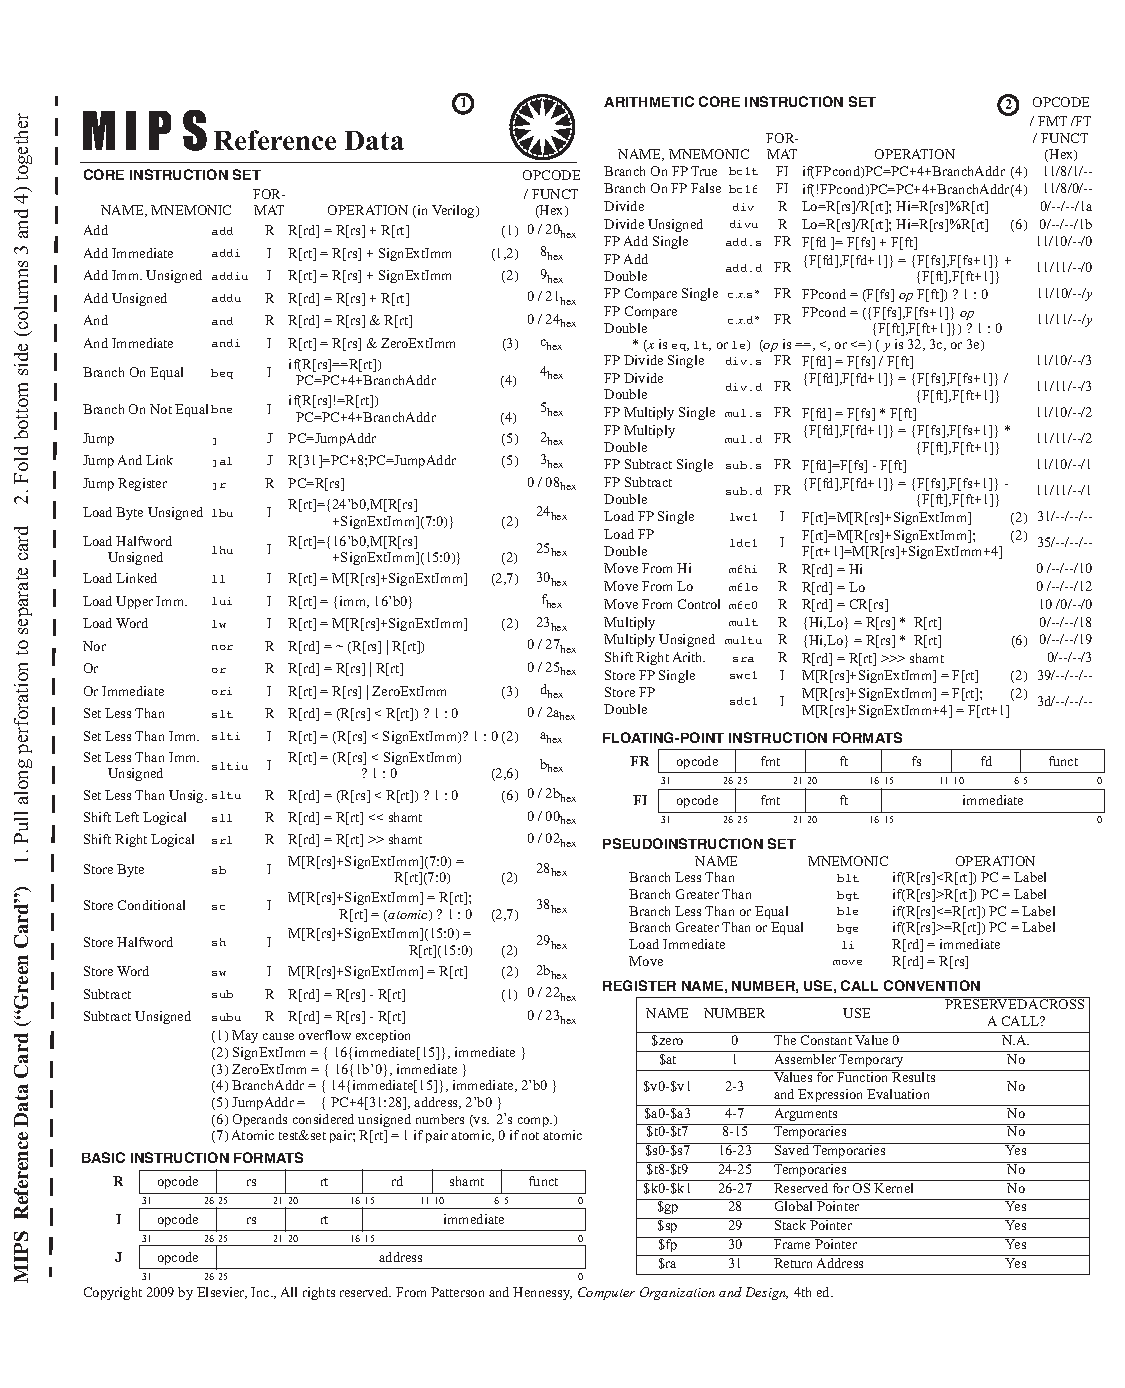
\includepdf[pages=-]{MIPS_Green_Sheet.pdf}
\showpoints
\end{document}
